
\section{Conclusions}\label{sec:Discussion}

This paper has made several findings. We have shown that modular predictors of object motion can be learned; that learning transfer is possible; that contact information assists transfer; that factorisation helps exploit this information; and that statistical machine learning can match or exceed tuned physics engine performance. The paper presented the first results on real objects for object transfer, and the first presentation of our modular-products scheme for prediction. What do these results tell us about the way to proceed? What is the space of methods for prediction? What promising avenues are there? We note the following issues.

\noindent {\bf Prior knowledge.} While the prior knowledge embodied by classical mechanics provides generality it prevents perfect prediction. Rigid body simulators need parameter learning, but have too few degrees of freedom to wrap themselves finely around real data. But we do need some structural knowledge: contact information is structural knowledge benefiting transfer. Pure tabula rasa learning is unlikely to be the answer. 

\noindent {\bf Local shape.} The learners used much less information than the full object shape. Further shape information can help. Local surface shape at contacts influences object motion. Experts specialised to local shape contexts would help, nesting another modular structure inside the product of experts, and solving the problem of how to attach experts to objects.

\noindent {\bf Modularity.} Modularity has credence in neuroscience, and is a good way to proceed for robots. Memory is cheap, and so learning many object specific modules is feasible. There is evidence that humans use modularity in developing expert motor skills. Modularity is part of the way to proceed.

\noindent{\bf Multiple changing contacts.}  In dextrous manipulation, the hand makes multiple and changing contacts with the object surface. Prediction for manipulation must therefore account for these non-smooth changes. It may be that hybrid models are a way to proceed.

\noindent {\bf Training noise.} Transfer performance degrades under training noise. We have partially addressed this by removing noise at prediction time using kinematic optimisation \cite{belter2014iros}. Whether this is extensible to other learning schemes is an open question.

\noindent{\bf Dynamics.} We have restricted this study to quasi-static cases, but the formulation of the basic regression problem with dynamics was given. Learning with dynamics is the next obvious step.

\newlength{\imgCXwid}
\setlength{\imgCXwid}{2.15cm}
\begin{figure*}[tbp]
%\centerline{
%\includegraphics[width=2.3cm]{images/C1_2exp_48_1}
%\includegraphics[width=2.3cm]{images/C1_2exp_48_2}
%\includegraphics[width=2.3cm]{images/C1_2exp_48_3}
%\includegraphics[width=2.3cm]{images/C1_2exp_48_4}
%\includegraphics[width=2.3cm]{images/C1_2exp_48_5}
%}
%\vspace{0.1cm}
\centerline{
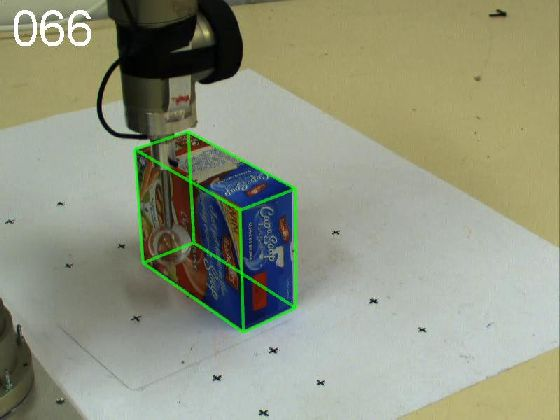
\includegraphics[width=\imgCXwid]{images/C1_2exp_87_1}
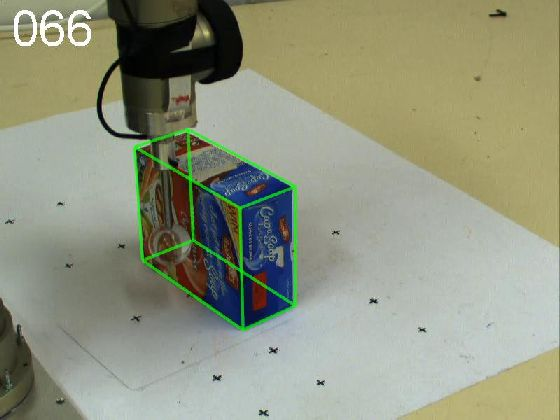
\includegraphics[width=\imgCXwid]{images/C1_1exp_87_1}
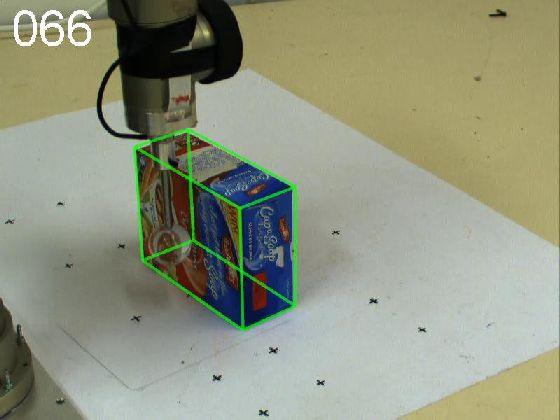
\includegraphics[width=\imgCXwid]{images/C1_LWPR1_87_1}
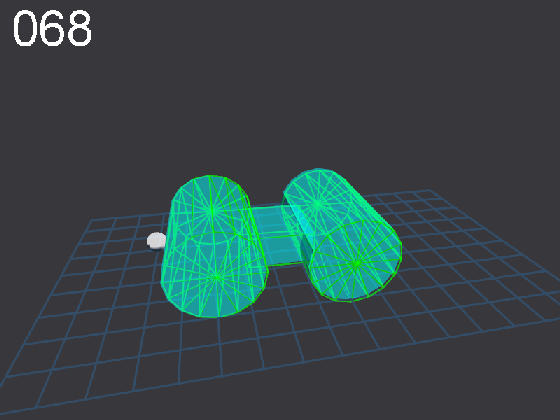
\includegraphics[width=\imgCXwid]{images/C5_1exp_6_1}
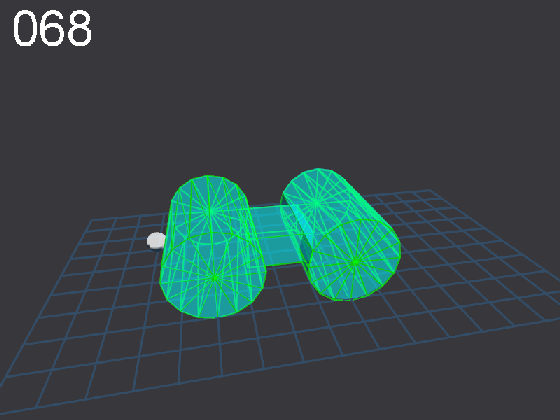
\includegraphics[width=\imgCXwid]{images/C5_2exp_6_1}
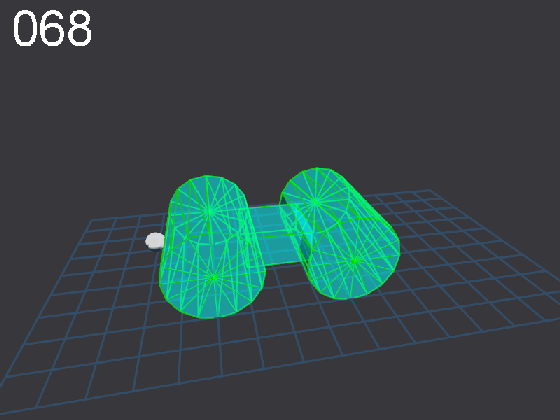
\includegraphics[width=\imgCXwid]{images/C5_3exp_6_1}
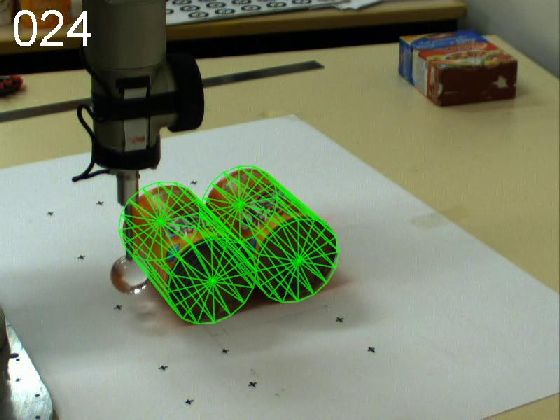
\includegraphics[width=\imgCXwid]{images/C2_3exp_75_1}
}
%\vspace{0.1cm}
\centerline{
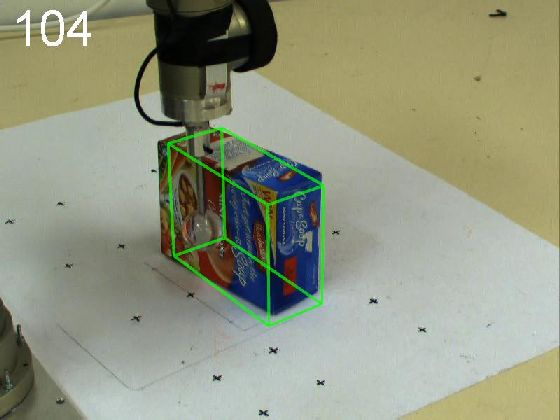
\includegraphics[width=\imgCXwid]{images/C1_2exp_87_2}
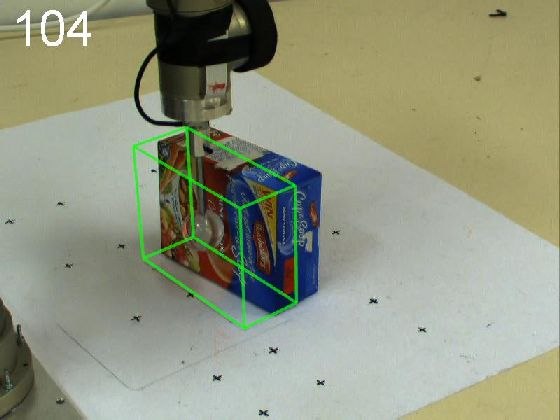
\includegraphics[width=\imgCXwid]{images/C1_1exp_87_2}
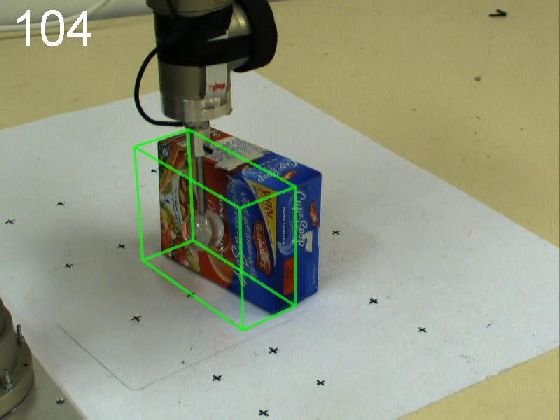
\includegraphics[width=\imgCXwid]{images/C1_LWPR1_87_2}
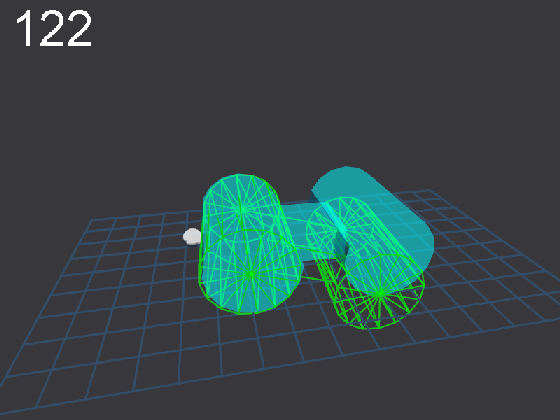
\includegraphics[width=\imgCXwid]{images/C5_1exp_6_2}
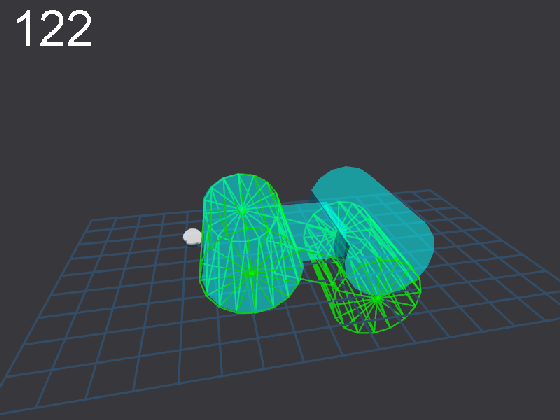
\includegraphics[width=\imgCXwid]{images/C5_2exp_6_2}
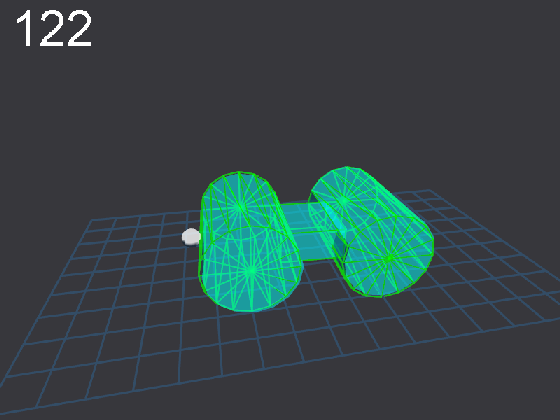
\includegraphics[width=\imgCXwid]{images/C5_3exp_6_2}
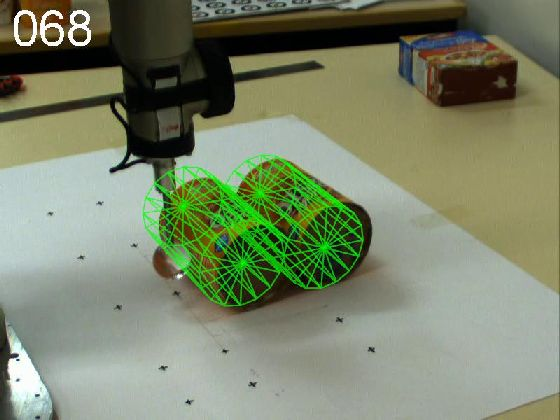
\includegraphics[width=\imgCXwid]{images/C2_3exp_75_2}
}
%\vspace{0.1cm}
\centerline{
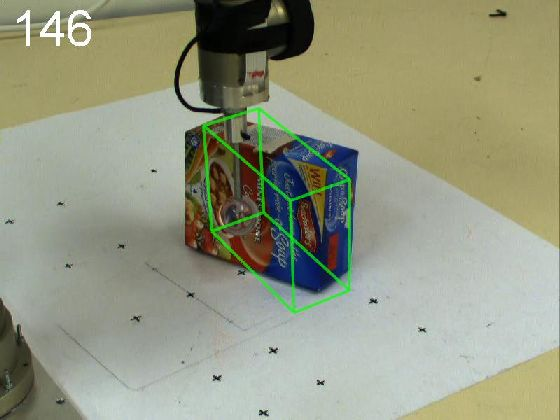
\includegraphics[width=\imgCXwid]{images/C1_2exp_87_3}
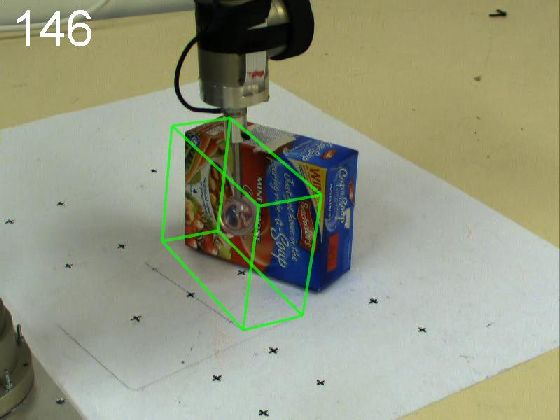
\includegraphics[width=\imgCXwid]{images/C1_1exp_87_3}
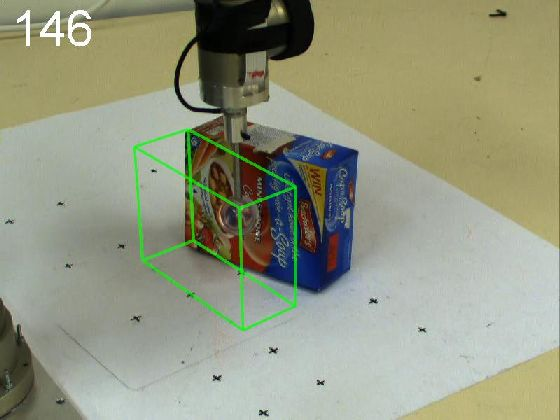
\includegraphics[width=\imgCXwid]{images/C1_LWPR1_87_3}
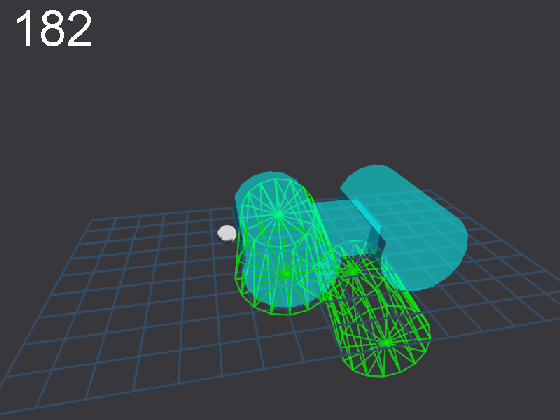
\includegraphics[width=\imgCXwid]{images/C5_1exp_6_3}
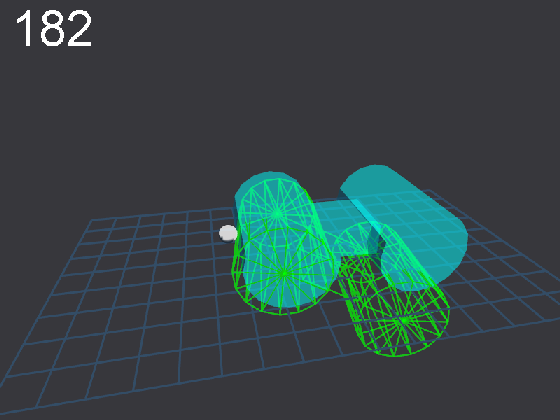
\includegraphics[width=\imgCXwid]{images/C5_2exp_6_3}
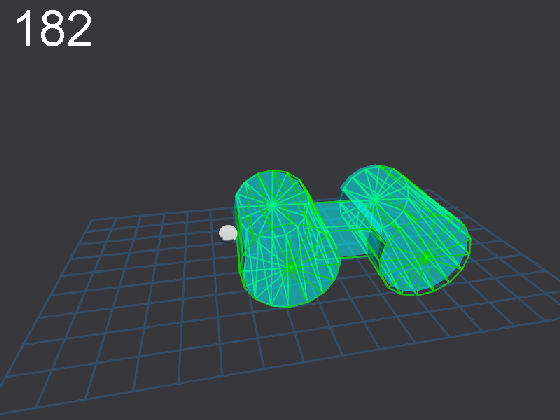
\includegraphics[width=\imgCXwid]{images/C5_3exp_6_3}
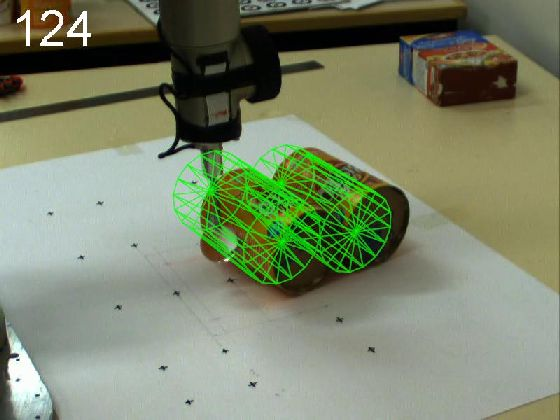
\includegraphics[width=\imgCXwid]{images/C2_3exp_75_3}
}
\centerline{
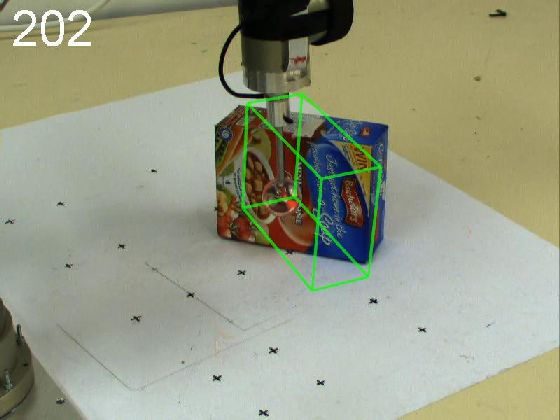
\includegraphics[width=\imgCXwid]{images/C1_2exp_87_4}
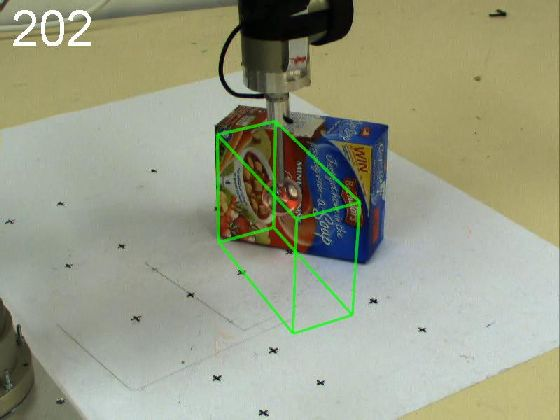
\includegraphics[width=\imgCXwid]{images/C1_1exp_87_4}
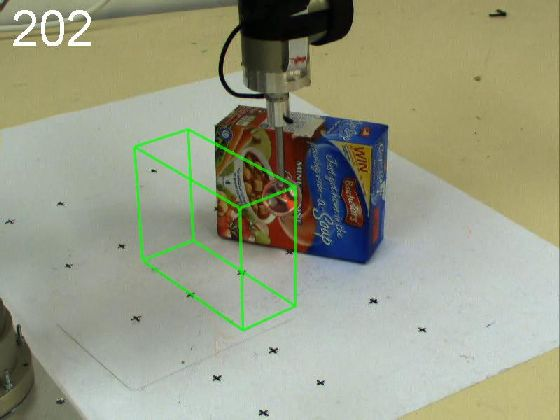
\includegraphics[width=\imgCXwid]{images/C1_LWPR1_87_4}
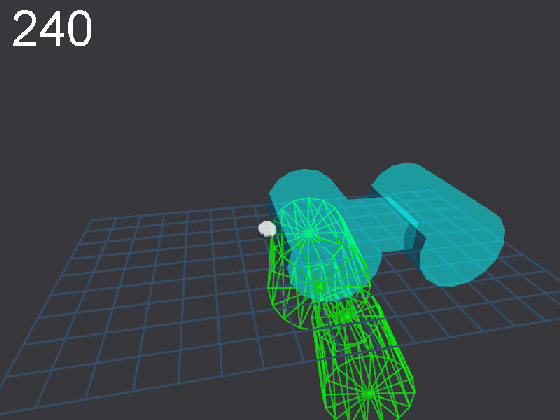
\includegraphics[width=\imgCXwid]{images/C5_1exp_6_4}
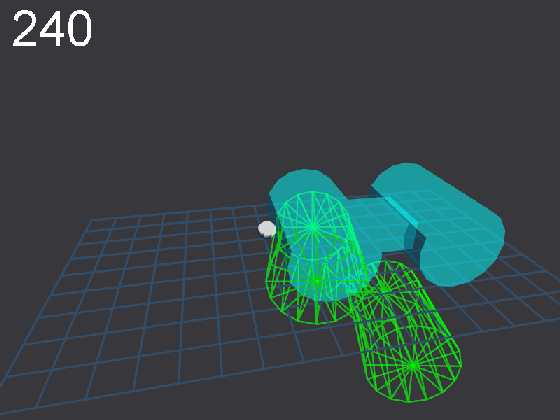
\includegraphics[width=\imgCXwid]{images/C5_2exp_6_4}
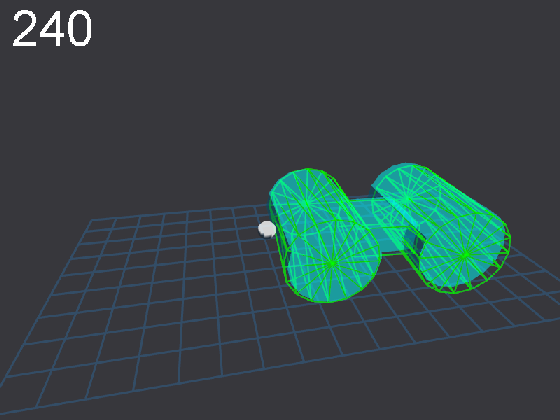
\includegraphics[width=\imgCXwid]{images/C5_3exp_6_4}
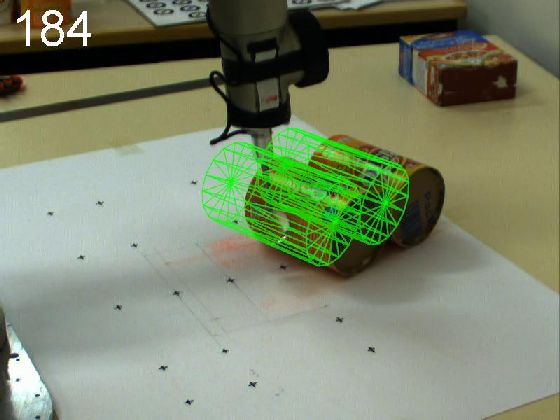
\includegraphics[width=\imgCXwid]{images/C2_3exp_75_4}
}
%\vspace{0.1cm}
\centerline{
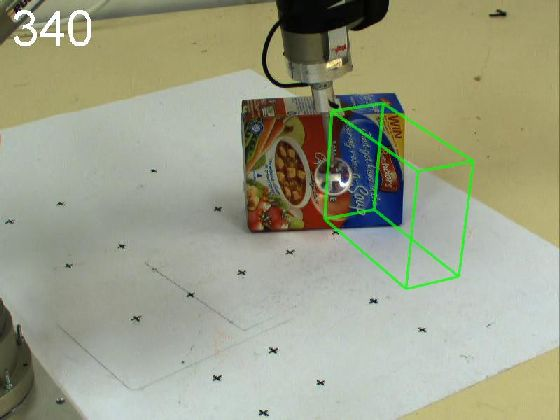
\includegraphics[width=\imgCXwid]{images/C1_2exp_87_5}
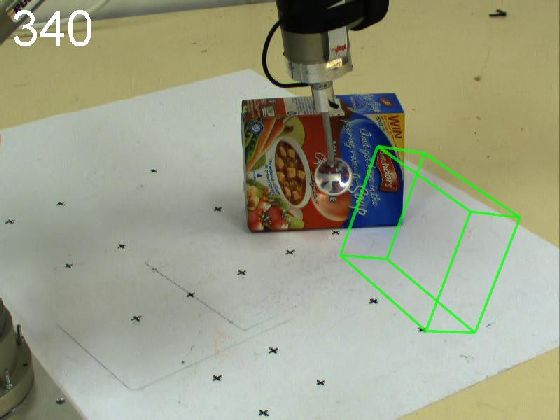
\includegraphics[width=\imgCXwid]{images/C1_1exp_87_5}
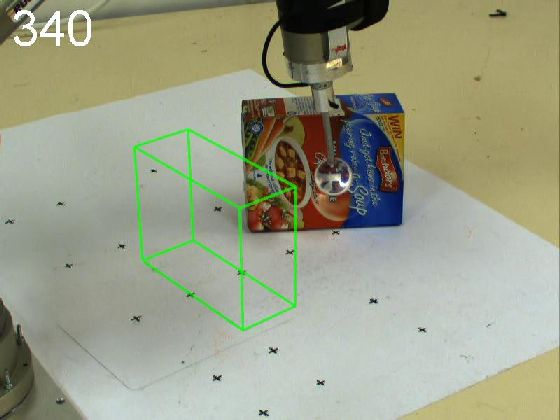
\includegraphics[width=\imgCXwid]{images/C1_LWPR1_87_5}
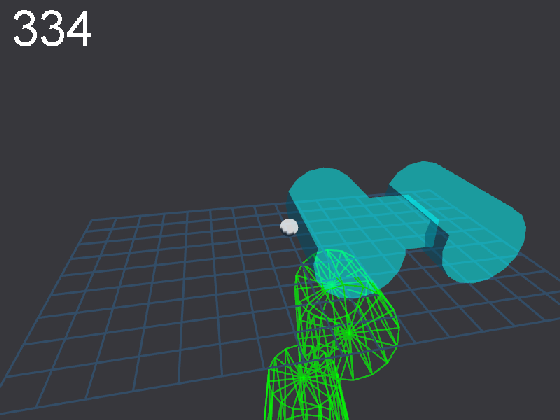
\includegraphics[width=\imgCXwid]{images/C5_1exp_6_5}
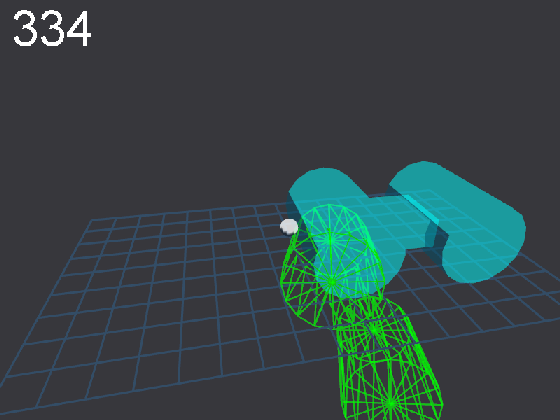
\includegraphics[width=\imgCXwid]{images/C5_2exp_6_5}
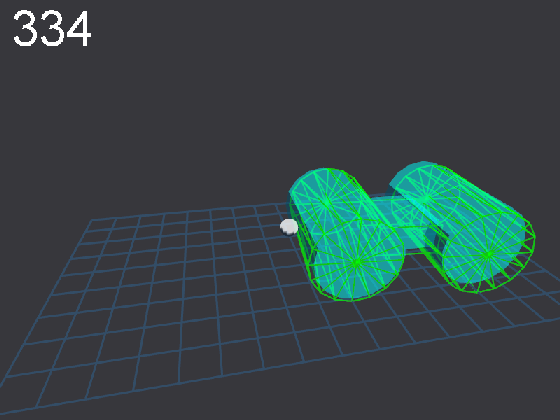
\includegraphics[width=\imgCXwid]{images/C5_3exp_6_5}
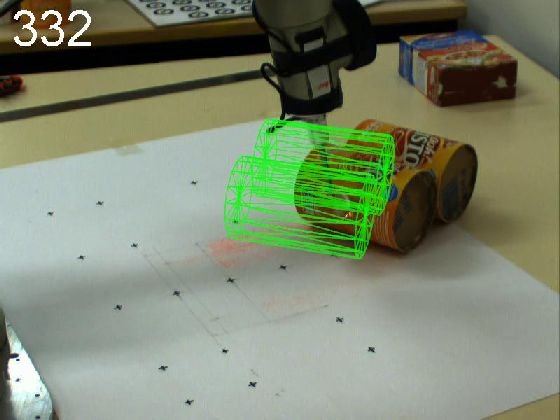
\includegraphics[width=\imgCXwid]{images/C2_3exp_75_5}
}

\caption {Experiment P3: Shape Transfer. Green outline shows predictions. Column~1: KDEF-GA/quat.
  Col~2: KDEF-G/quat. Col~3: LWPR-G for one trial.  Note that the
  KDEF-G/quat and LWPR-G methods predict that the robot finger moves
  into the box.  Col~4: KDEF-G/quat. Col~5: KDEF-GA/quat. Col~6:
  KDEF-GAE/quat. Col~7: KDEF-GAE/quat. The frame number is shown in
  the top left of each image.  }
\label{fig:ExperimentStransfer}
\end{figure*}

%This paper has sought to establish a case for modular, machine learning approaches to metric prediction as a promising alternative to analytic modelling. Essentially machine learning plus modularisation allows us to predict accurately in the face of unobservable parameters. Unlike other learning approaches, ours provides precise predictions of rigid body motion over many steps, and can transfer predictions to novel actions and objects. This required exploiting the insight from analytic modelling that each contact must be modelled explicitly, and the structure of the learner should reflect the contact structure so as to to exploit this information. In summary combining insights from analytic and machine learning approaches is, we believe, the way forward.
